\chapter{Data acquisition and preprocessing}

Having reliable data is a fundamental requirement in building a good model. In this chapter we describe the data measurement setup and the data acquisition process used in capturing the dataset used for surface classification. 

\section{Datacubes and datasquares}
Some radars have antennas providing multiple simultaneous outputs. In such systems each transmitted pulse generate a two-dimensional image as $P$ recievers each collect $L$ range  samples. Collecting $Q$ sequential pulses produce a \emph{datacube} containing $P\times L\times Q$ samples \citep{richards_2014}. This intuitively pleasing representation of data acquired by a radar array is commonly referenced in journal papers when describing for instance beam forming or doppler processing algorithms \citep{gentile_donovan_2018}. As described in chapter 2, range estimates are formed from estimating the time-of-flight of a returning wavelet from a target scene. This process forms the shortest time frame possible with resolutions on the picosecond scale for millimeter-wave radar, and is because of this commonly referred to as the \emph{fast time} scale. Conversely, the dimension consisting of full sets of range measurements is known as the \emph{slow time} scale.

In this report one dimensional sensors are used, rendering \emph{data squares} with fast time and slow time axes, but no sensor axis, of sizes $L\times Q$ (A more appropriate name would perhaps be call these data rectangles, but since their three dimensional counterparts are not named data cuboids they are hereby referred to as squares).  

In this work two sensors collect data in parallel. During one run, or one \emph{session}, one datasquare is captured per sensor. As the two sensors used in this project are not synchronized we are unable to form the third dimension described above and may just as well concatenate the two existing ones to form one larger datasquare. If the contents of the two datasquares are described as $r_1(d,t)$ and $r_2(d,t)$ with fast time sample $d$ and slow time sample $t$, the larger concatenated datasquare matrix $\mathbf{R}$ can be formed as

\begin{equation}
	\mathbf{R}= 
	\begin{bmatrix}
		r_1(0,0) & r_1(1,0) & \cdots & r_1(N,0) & r_2(0,0) & \cdots & r_2(N,0) \\
		r_1(0,1) & r_1(1,1) & \cdots & r_1(N,1) & r_2(0,1) & \cdots & r_2(N,1) \\
		\vdots &  \vdots & \ddots & \vdots & \vdots & \ddots &  \vdots \\
		r_1(0,Q) & r_1(0,Q) & \cdots  & r_1(N,Q) & r_2(0,Q) & \cdots  & r_2(N,Q) \\
	\end{bmatrix}
	,
\end{equation}

or, more succinctly, as samples $r(n,t) = \mathbf{R}_{n,t}$. Each session is built up of 50,000 slow time samples, so that $t=1,\,...\,,50000$.

\section{Measurement Setup}

% There are many parameters to consider in optimizing the data collecting process, and often an endless amount of possible configurations among these. This can make it impossible to find an optimal solution, but putting some thought into every decision can prove worthwhile. Below, we motivate our choices of sensor placement as well as various parameters.

% After this is done, the data is collected by recording radar sweeps at a certain rate while moving across a surface, according to figure \ref{fig:data_collecting}.

As mentioned above, two sensors each capture one datasquare per session in the collection process. Sensor data is acquired while the robot is moving at a constant pace, illustrated in figure \ref{fig:data_collecting}. Furthermore, two mounting angles are used, where one sensor is facing directly towards the ground, while the other has a round $22.5^\circ$ tilt forward. The reasoning behind this setup is for each sensor to capture different aspects of the surface below; the flatly placed sensor captures a larger component of the specular (mirror-like) scattering process from the ground plane, while the tilted captures more of the non-specular scatterers. 

This idea is illustrated in figure \ref{fig:reflections}. If we are presented with two surfaces of the same material but with different ruggedness, the two will still scatter differently in spite of their equivalent dielectric properties. The scattering processes considered in this work should be highly dependant on the surface structure, where the predictability, or the randomness, should vary from material to material. It is worth noting that the angular spread of the sensor is roughly $30^\circ$ \citep{acconeer_datasheet_a111}, meaning that a $60^\circ$ angle from the sensor is illuminated at once. 

\begin{figure}[h]
	\centering
	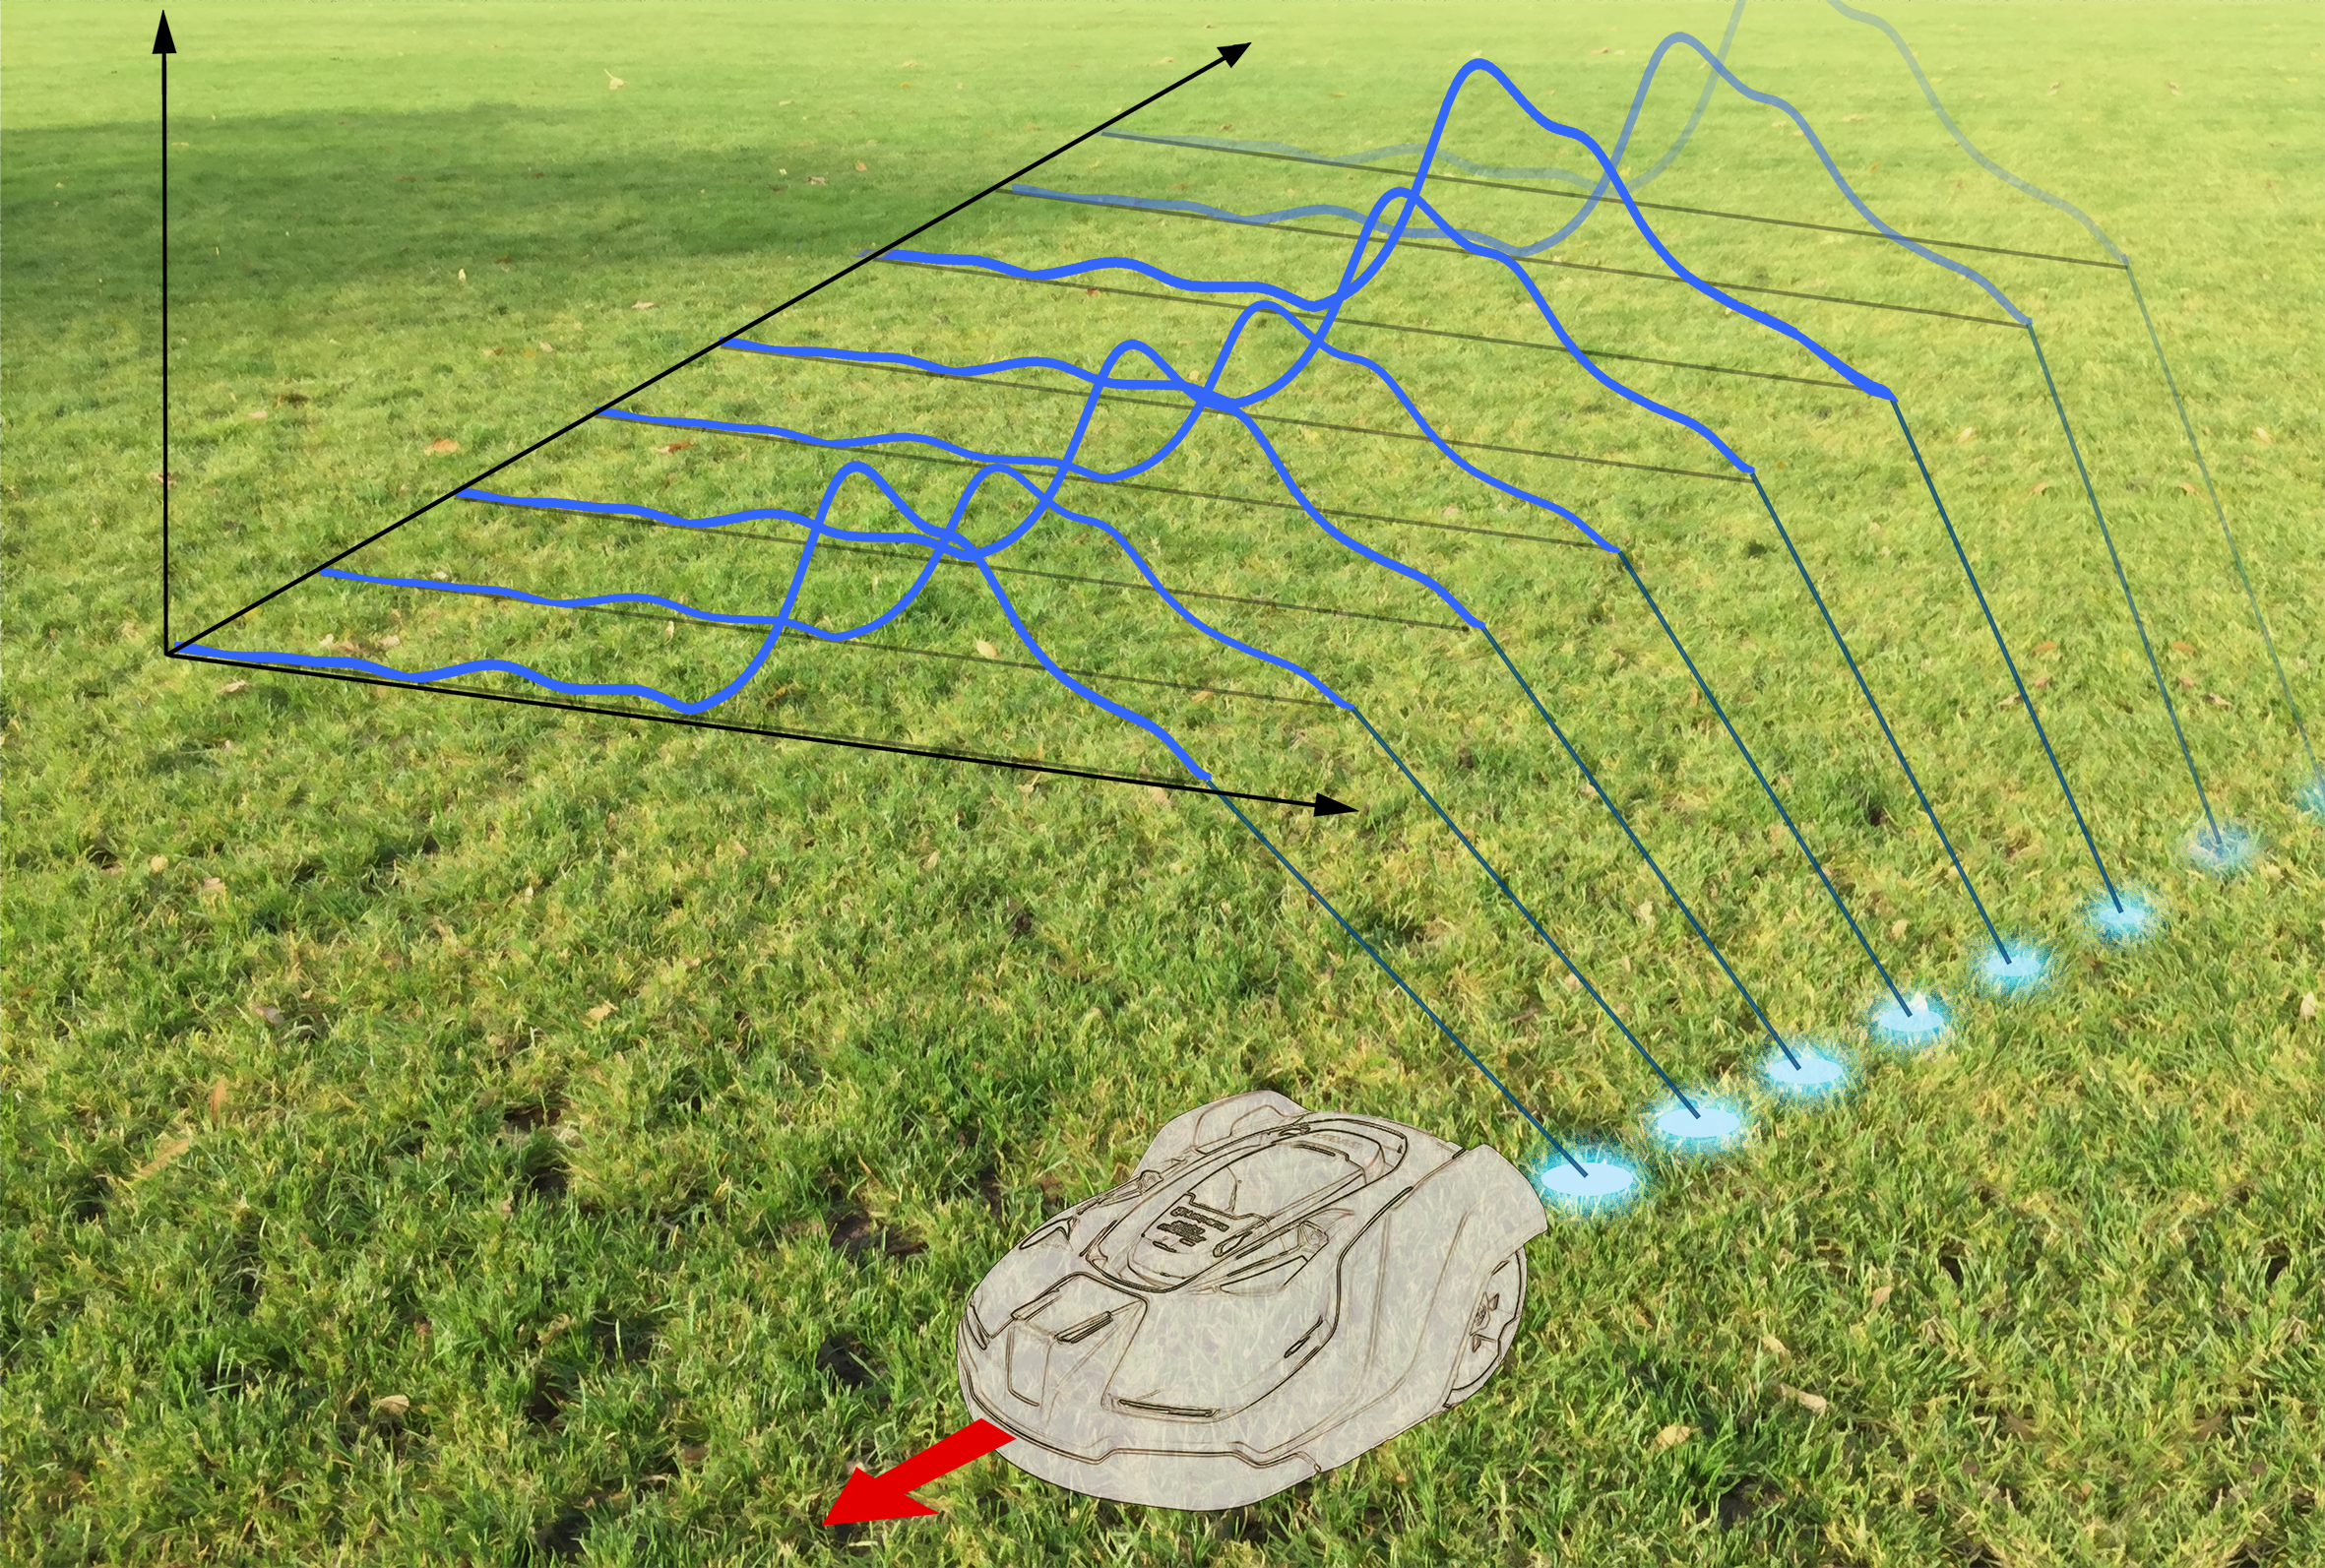
\includegraphics[scale=0.60]{figs_temp/data_collecting.jpg}
	\caption{Two sensors mounted at the front of a robot collect data while the robot is moving forward. Note that the collected data is of IQ-form, whereas the image depicts its absolute values for the sake of clarity.}
	\label{fig:data_collecting}
\end{figure}

%The measurement setup is comprised of two sensors, mounted at the front of a slowly moving robot. One of the sensors is facing straight down towards the ground, whereas the other one is tilted 22.5 degrees, facing forward. The idea behind this setup is that the two sensors will capture information about the same surface but from different directions. 


%Say for example we are presented two surfaces with equivalent reflective properties but where one is rugged and the other is smooth. For the smooth surface the reflections behave more predictably than those for the rugged. If a strong electromagnetic pulse is transmitted from the sensor facing down, one would expect to receive a strong response from the smooth surface. If one instead were to transmit a pulse from the tilted sensor, a weak response would rather be expected due to the specular reflection atop the, ideally, flat surface. 

%For the rough surface on the other hand, the signal would scatter in a wider array of angles, both when the pulse is transmitted from the flat and the tilted sensor. An idealization of what the received reflection amplitudes could look like from the four scenarios (2 surfaces, and 2 sensors) is presented in figure \ref{fig:reflections}.

\begin{figure}[h]
	\centering
	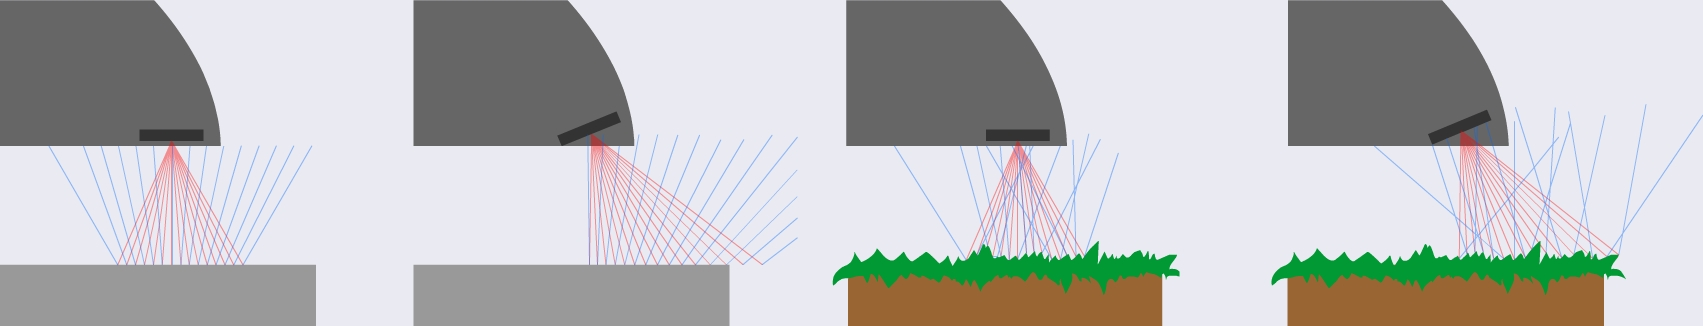
\includegraphics[scale=0.9]{figs_temp/reflections.jpg}
	\caption{Using two sensors mounted with different tilts, we can get information about a surface's roughness. For a smooth surface, the flat and tilted sensors yield a very different response, whereas for a rugged surface the responses are more similar.}
	\label{fig:reflections}
\end{figure}

A final consideration is that as the sensors are placed on the inside of the robot plastic chassis, there is a risk for interference between in the region between the plastic and the antenna. To avoid this a small mount was 3D-printed so that the distance to the plastic was $\lambda/4$. Doing this means that any waves propagating back and forth in this region interfere destructively due to the change in polarity and the superposition principle of electromagnetic radiation \citep{griffiths_2018}.

\section{Measurement Settings}

The Acconeer radar system has a number of settings controlled by the user. In this section a few key parameters of these are discussed, namely the distance interval sampled, the sampling frequency and the wavelet size. Although finding the appropriate sensor settings requires some level of trial-and-error due to hardware and software limitations, a good starting point can be found using a theoretical perspective. 

%Setting the sensor parameters is an iterative process which requires a trial-and-error approach. However, the choices for some parameters can be narrowed down with a little bit of thought.

When working with radars and moving targets it is important to select a frequency capable of resolving the maximum speed of the target. If a too low frequency is used, aliasing occurs distorting the frequency spectrum \citep{lindgren_rootzeŽn_sandsten_2013}. In order to assure that aliasing does not occur, one must select a sampling rate $f_s$ at least twice the received maximal frequency component $f_{max}$. This limit, commonly known as the Nyquist limit \citep{proakis_manolakis_1995}, thus places the requirement on the sampling frequency that 

\begin{equation}
\label{eq:nyquist}
		f_{s} \geq 2f_{max}.
\end{equation}
The sampling frequency should therefore be chosen with regards to the maximal frequency component present in the signal. 

In figure \ref{fig:sensor_placement}, a vehicle is moving forward with constant speed, $v_0$, having a sensor mounted at the front with a 22.5 degree tilt, and a 60 degree angular spread. As it moves forward, the ground moves past the radar sensor at a velocity $v_0$. The maximal velocity component that is orthogonal to the sensor occurs at the far end of the radar's view at $22.5^\circ + 30^\circ = 37.5^\circ$ tilt. 

The movements orthogonal to the radar give rise to doppler frequencies $f_d$ related to the speed towards the sensor $v_\perp$ according to \citep{lien_gillian_karagozler_amihood_schwesig_olson_raja_poupyrev_2016}

\begin{equation}
	f_{d} = \frac{2v_\perp}{\lambda}.
\end{equation}
With $v_0=0.3$ m/s and $\lambda = 2\pi/\Omega = 0.005$ m, the maximal doppler frequency that can occur is given by 
\begin{equation}
	f_{d,\textrm{max}} 
	=\frac{2 v_{\perp, \textrm{max}}}{\lambda} 
	= \frac{2 v_0\cos(37.5^\circ)}{\lambda}
	\approx 95.2 \text { Hz}.
\end{equation}
Combining this result with equation \eqref{eq:nyquist}, we see that we have to select  a sampling frequency that satisfies
\begin{equation}
	f_s > 2f_{d,\textrm{max}} = 190.4 \text{ Hz}.
\end{equation}

The transmitted constant-frequency wavelet has three main properties: Its amplitude, its frequency and its duration. Generally, the amplitude is set as high as possible, simply because the signal-to-noise ratio is increased \citep{richards_2014}. The frequency is essentially set for the system used at around 60 GHz without any significant leeway. The duration may however be chosen somewhat freely. Selecting a longer wavelet means transmitting more energy and thus receiving a signal with better SNR. A shorter wavelet has worse SNR, but is capable of resolving finer details of the target. Thus, the wavelet duration parameter becomes a tradeoff between resolution and SNR. Thus, one may start with a short wavelet and increase its duration until a reasonable SNR is obtained.  

Finally, the distance interval measured has to be chosen. Again, a tradeoff appears. If a short interval is selected we can increase the sampling rate and still stay within the allowed hardware transmission speed limits. However, if the interval becomes too short we may miss useful information we could have collected outside the chosen interval. Thus, a reasonable strategy is to select the most critical range interval and then increase the sampling frequency to its hardware allowed limit. As the distance to the surface plane was roughly 12 cm the furthest distance illuminated is $12/\sin(37.5^\circ)\approx 20$ cm. We should therefore at least have a range spanning this region.  

The values chosen for the three parameters are summarized in table \ref{tab:sensor_settings}. 

\begin{table}
\begin{center}
	\begin{tabular}{|c|c|}
	  	\hline
	  	\cellcolor{gray!150}\color{white}\textbf{Setting} & \cellcolor{gray!150}\color{white}\textbf{Value} \\
	 	 Wavelet duration & 50 ps \\
	  	\cellcolor{gray!25}Sampling frequency & \cellcolor{gray!25}200 Hz \\
	  	Range interval & 7 to 23 cm \\ 
		\hline
  	\end{tabular}	
\end{center}
\caption{Sensor settings.}
\label{tab:sensor_settings}
\end{table}



\begin{figure}[h]
	\centering
	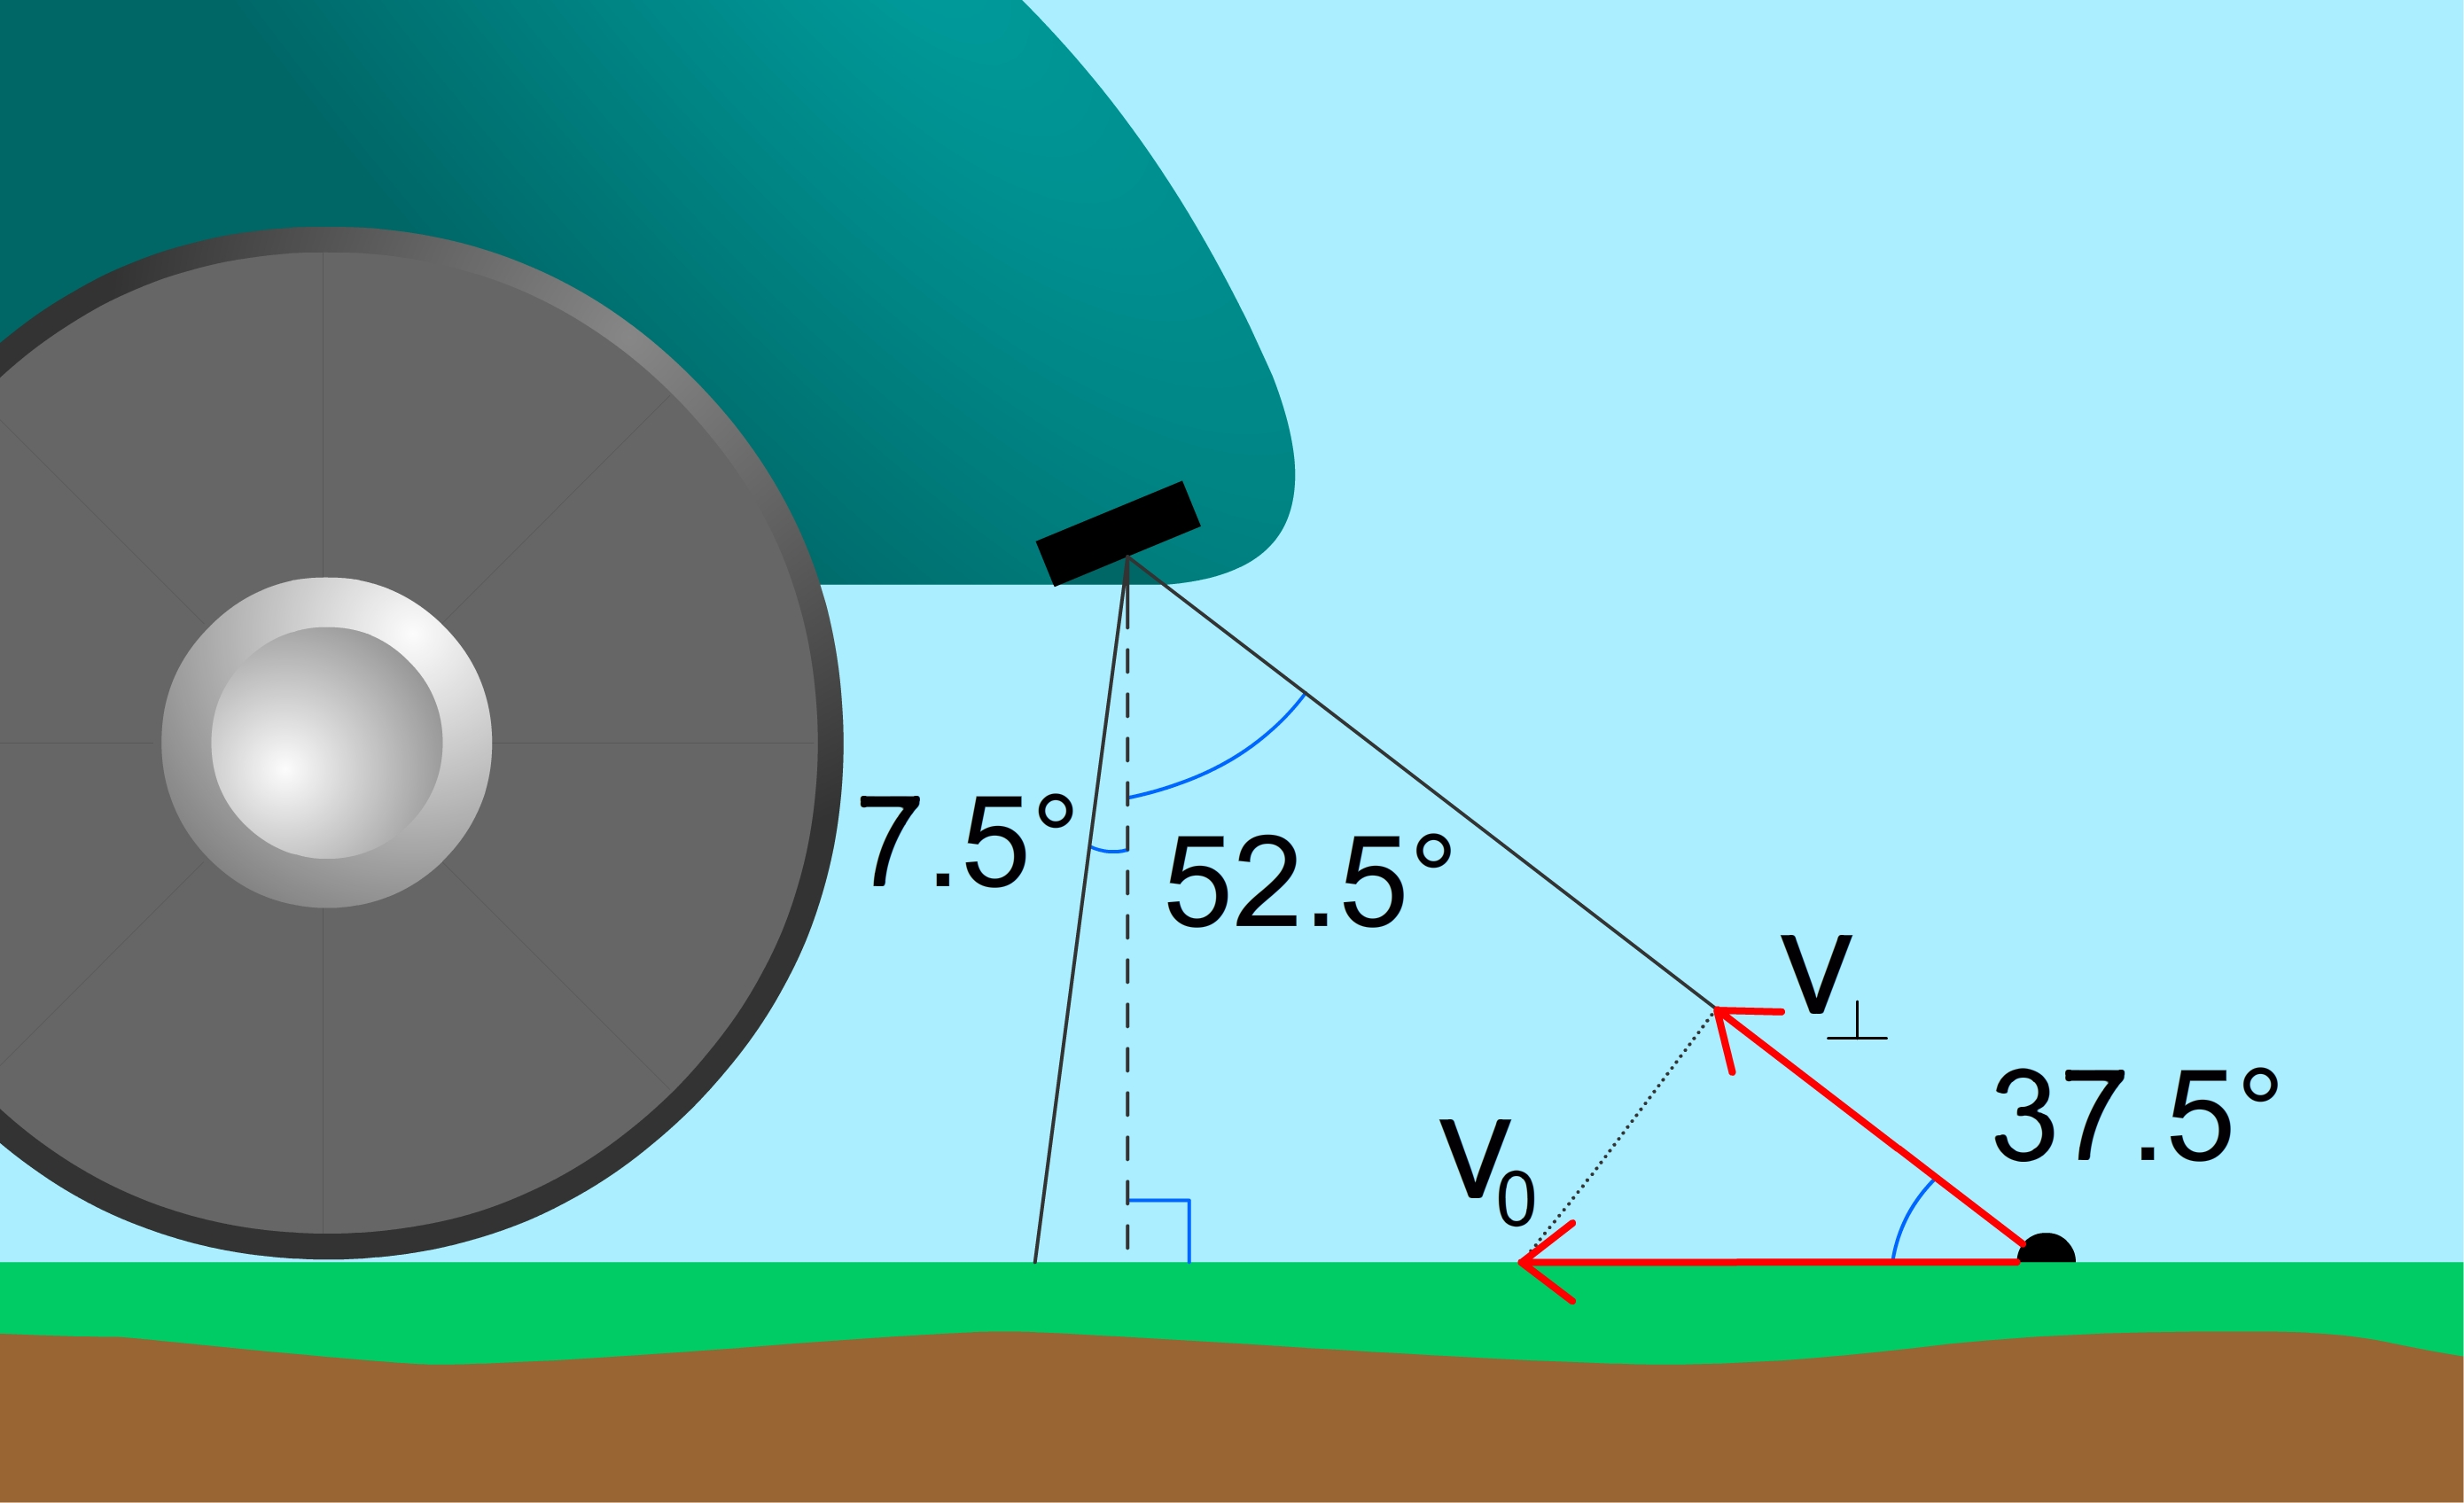
\includegraphics[scale=0.30]{figs_temp/sensor_placement.jpg}
	\caption{}
	\label{fig:sensor_placement}
\end{figure}

%\section{Data Preprocessing}
\section{Downsampling}

In an information theoretic framework we interpret a random variable by how unpredicable or unstructured an observation of the variable is\citep{anderson_johnnesson_2006}. First introduced by Claude E. Shannon in his famous 1948 papers, information theory brings about a mean to quantify the information content of some source \citep{shannon_1948}. This concept, which essentially concerns examining the randomness of a variable, is commonly measured through entropy. Directly related to entropy is mutual information which asserts how much information each member of a set have on the other members. \citep{hyvasrinen_karhunen_oja_2004}. Ideally one wants measurements that have a low measure of mutual information, meaning that each datapoint contain information not found elsewhere in the set. 

Observing a typical radar sweep in figure \ref{fig:single_sweep_iq} we note that points are very closely related on a small range scale, and nearly identical if we were to examine them on a sample by sample basis. One could argue that the mutual information found in the set is very high and that the entropy in each datapoint is low. Hence, to lower the first and increase the latter, one could downsample by some factor $D$ in range without significant loss of information.

Downsampling measurements $r_1(d,t)$ and $r_2(d,t)$ by a factor $D$ can be expressed as

\begin{equation}
	r_{1,D}(d, t) = r_{1}(dD,t), 
	\quad \text{and} \quad r_{2,D}(d,t) = r_{2}(dD,t)
\end{equation}

and the datasquare $r_D(n,t)$ is formed correspondingly.

\section{Sweep Normalization}

Radar gain can vary significantly from one sensor to another. This means that faced the same surface, two sensors may exhibit a similar sweep structure but with differing amplitudes. Assuming a model's training data has been collected with one sensor, it could therefore perhaps be difficult to successfully perform classifications with the same model using a sensor which has a different gain. This is due to the fact that a linear scaling difference between two sensors behaves nonlinearly in the prediction output, due to nonlinearities both in the feature extraction process as well as in the classification process.

A way to overcome this issue is to perform sweep normalization as a preprocessing step. There are multiple ways of performing such a normalization. A simple strategy is to simply divide each sweep with its maximum absolute value. While this may intuitively seem like a good idea, it eliminates certain signal evolution structures between consecutive captured sweeps - if three consecutive sweeps vary in received signal strength we wish to capture such a behaviour. 

A better solution is to instead have the normalization method depend on several consecutive sweeps. By computing the average energy in all range bins and over a number of sweeps, we can instead normalize using this value, and thus maintain some of their relative structure. Constructing one \emph{data batch} $m$ consisting of $r_D(n,mT + \tau)$ for $\tau=0\text{ }...\text{ }T-1$ for $T$ consecutive sweeps, we can average over the energy content in the entire batch to form scaled, downsampled data $x(n,m,\tau)$ through

\begin{equation}
	x(n,m,\tau) = 
	\frac{r_{D}(n,mT + \tau)TK}
	{\sum_{n=0}^{K-1}\sum_{\tau=0}^{T-1}|r_{D}(n,mT + \tau)|}.
\end{equation}

While this particular method to form data batches $x(n,m,\tau)$ may seem odd at this point, we will see in the following chapter that it makes a lot of sense in the feature extraction framework used.
